\documentclass[12pt]{article} %Basic document type
\usepackage{times} %Font 
\usepackage{amsmath} %For matrices
\usepackage{amssymb}
\usepackage[section]{placeins} %Allows FloatBarrier command
\usepackage[utf8]{inputenc} %Font encoding
\usepackage[margin=1.25in]{geometry} %Adjust margins
\usepackage{graphicx} %Allows picture import
\usepackage{pdfpages} %Including pdf files 
\usepackage{setspace}
\usepackage{fancyhdr}
\usepackage{appendix}
\graphicspath{{images/}} %Allows picture impor
\pagestyle{fancy}
\fancyhf{}
\fancyhead[L]{A Real-Time Object Tracking System}
\fancyhead[R]{ECSE 456}
\fancyfoot[C]{\thepage}
\renewcommand{\headrulewidth}{1pt}
\renewcommand{\footrulewidth}{1.5pt}
\newcommand{\HRule}[1][\medskipamount]{\par
  \vspace*{\dimexpr-\parskip-\baselineskip+#1}
  \noindent\rule{\linewidth}{0.2mm}\par
  \vspace*{\dimexpr-\parskip-.5\baselineskip+#1}}
\begin{document}
\begin{titlepage}
\begin{center}
\textsc{\huge McGill University}\\[1.5cm]
\textsc{\LARGE Department of Electrical \& Computer Engineering}\\[1.5cm]
\textsc{\Large ECSE 456 - Final Report}\\[3cm]
\HRule
{\huge \bfseries A Real-Time Object Tracking System \\[.3cm] }
\HRule 
\vspace{1.5cm}
\noindent
\begin{minipage}{0.4\textwidth}
\begin{flushleft} \large
\emph{\Large Authors:}\\
\vspace{.2cm}
Benjamin \textsc{Brown} \\
\textit{benjamin.brown2@mail.mcgill.ca} \\
260450182 \\
\vspace{.2cm}
Taylor \textsc{Dotsikas} \\
\textit{taylor.dotsikas@mail.mcgill.ca} \\
260457719
\end{flushleft}
\begin{flushleft} \large
\emph{\Large Supervisors:}\\
\vspace{.2cm}
Warren \textsc{Gross, Prof.}\\
\vspace{.2cm}
Arash \textsc{Ardakani} 
\end{flushleft}
\end{minipage}%
\end{center}
\end{titlepage}
\pagebreak
\section*{Abstract}
Video processing represents an extremely relevant challenge as both the demand for intelligent, aware systems and the quality of modern video technology increases. This increase in quality comes at a cost of large amounts of data being handled under strict time constraints \cite{3}. This project aimed to study how a common video processing algorithm such as object motion tracking can be accelerated using custom hardware. This report concludes on the background, design, and findings of Phase 1 of the project; where platform research, algorithm research, and software implementation was performed. It was clear that an FPGA would be the best solution for fast, low power hardware implementation and a Kalman filter based algorithm was the best solution for a predictive algorithm not prone to noise. Finally, the large amount of time the software needed to process relatively short videos proved that direct hardware implementation of the algorithm is essential for applications. 
\section*{Acknowledgments}
The authors would like to thank Professor Warren Gross, for undertaking the responsibility of supervising this project. We would also like to thank Arash Ardakani for all of his advice, help, and time spent meeting with us throughout the semester. Finally, we would like to thank anyone who contributed to the wealth of online resources about object tracking that we hope to contribute to.
\pagebreak
\tableofcontents
\pagebreak
\section{Abbreviations \& Notation}
\begin{itemize}
\item[] FPGA - Field Programmable Gate Array
\item[] ASIC - Application Specific Integrated Circuit
\item[] CPU - Central Processing Unit
\item[] DFG - Delta Frame Generation
\end{itemize}
\section{Introduction}
\subsection{Motivation}
Scene recreation and analysis is imperative in digital systems that must understand and react to events in their environment. Some typical examples of this include surveillance, robotics, and human-computer interaction. A variety of sensors can be employed for such a task including ultrasonic, radar, and passive infrared, but all of these sensors do not come close to modeling an environment as completely as a video camera. With the increase in image quality and device accessibility, the video camera seems like the obvious solution. \\\\
However, due to the vast amount of data and system imposed processing time constraints, video processing is a challenge. For instance, the transition to a high-definition video platform produces six times more data than the previous standard-definition one \cite{3}. This project aims to study how a complex video processing algorithm such as real-time object tracking can be greatly accelerated when implemented directly in hardware. Object tracking represents an excellent example of the aforementioned challenges because it requires capturing an image of a scene, processing the image to locate the object in motion, and reconstructing said scene with emphasis placed on the motion, all in real-time.
\subsection{Applications}
Taylor
\section{Background}
\subsection{Video Processing}
Ben 
\subsection{Optical Flow}
Ben (general) \& Taylor (DFG)
\subsection{Kalman Filter}
Ben
\subsection{Fixed vs. Floating-Point}
Ben
\section{Requirements}
Taylor
\section{Design}
Ben \& Taylor
\subsection{Algorithm}
\subsection{Software}
\begin{figure}[h]
\centering
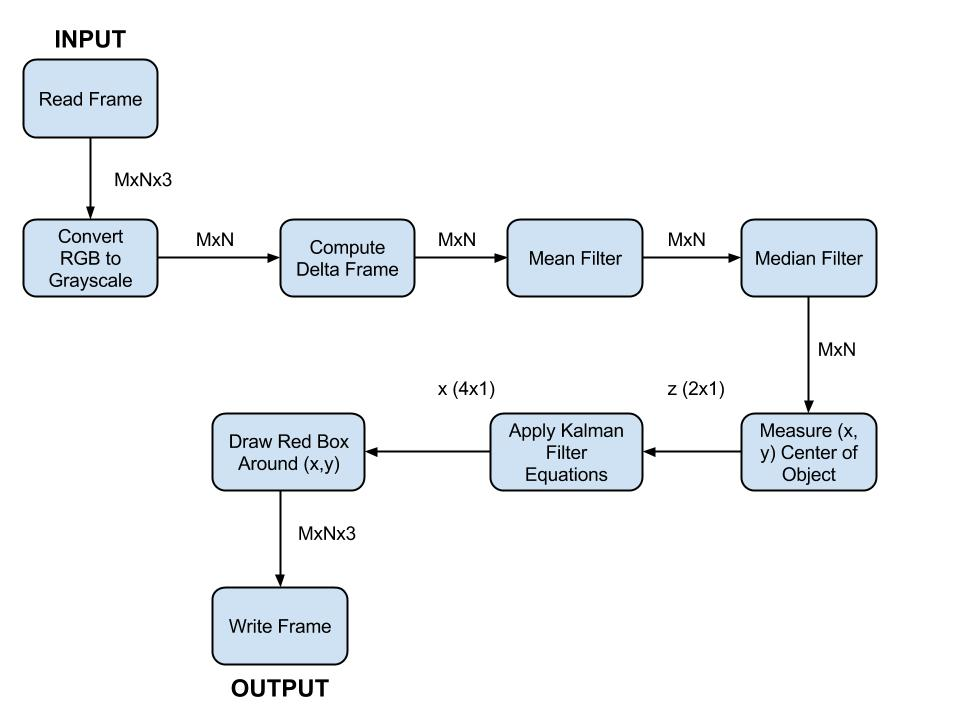
\includegraphics[width=0.75\textwidth]{./images/software_flow.jpg}
\caption{Software Flowchart}
\label{fig:sw_flow}    
\end{figure}
\section{Future Work}
Ben \& Taylor
\section{Impact on Society}
Taylor
\section{Allocation of Work}
Ben \& Taylor
\section{Conclusion}
Ben \& Taylor
\newpage
\begin{thebibliography}{11}
\bibitem{1}
F. Roth, “Using low cost FPGAs for realtime video processing”, M.S. thesis, Faculty of Informatics, Masaryk University, 2011.
\bibitem{2}
A. Saeed et al., “FPGA based Real-time Target Tracking on a Mobile Platform,” in 2010 International Conference on Computational Intelligence and Communication Networks, 2010, pp. 560-564.
\bibitem{3}
”Video and Image Processing Design Using FPGAs.” Altera. 2007. January 2014. 
http://www.altera.com/literature/wp/wp-video0306.pdf  
\bibitem{4}
E. Trucco and A. Verri, “Chapter 8 - Motion,” in Introductory Techniques for 3D Computer, pp. 177- 219.
\bibitem{5}
S.A. El-Azim et al., “An Efficient Object Tracking Technique Using Block-Matching Algorithm”, in Nineteenth National Radio Science Conference, Alexandria, 2002, pp. 427 - 433.
\bibitem{6} 
Caner et al., “An Adaptive Filtering Framework For Image Registration”, IEEE Trans. Acoustics, Speech, and Signal Processing, vol. 2, no. 2, 885-888. March, 2005. 
\bibitem{7}
Yin et al. \textit{Performance Evaluation of Object Tracking Algorithm} [Online]. Available: http://dircweb.kingston.ac.uk/ 
\bibitem{8}
G. Shrikanth, K. Subramanian, “Implementation of FPGA-Based object tracking algorithm,” Electronics and Communication Engineering Sri Venkateswara College of Engineering, 2008.
\bibitem{9}
E. Pizzini, D. Thomas, “FPGA Based Kalman Filter,” Worcester Polytechnic Institute, 2012.
\bibitem{10}
M. Shabany. (2011, December 27). \textit{Floating-point to Fixed-point Conversion} [Online]. Available: http://ee.sharif.edu/~digitalvlsi/Docs/Fixed-Point.pdf
\bibitem{11} 
N. Devillard. (1998, July). \textit{Fast median search: an ANSI C implementation} [Online]. Available: http://ndevilla.free.fr/median/median.pdf
\end{thebibliography}
\newpage
\appendix
\appendixpage
\section{Additional Figures} \label{sec:add}
\end{document}